\documentclass[mathserif, handout]{beamer}
% ======================================================================
% General LaTeX Setup for Beamer (Reusable Preamble)
% Author: Chandra Gummaluru
% ======================================================================

\documentclass[mathserif, handout]{beamer}
\setbeamertemplate{frametitle}{}

% ------------------------------------------------------------
% basic packages
% ------------------------------------------------------------
\usepackage{url}
\usepackage{ifthen}
\usepackage{enumerate}
\usepackage[font=small]{caption}
\usepackage{subcaption}
\usepackage{moresize}
\usepackage[outline]{contour}
\usepackage{transparent}
\usepackage{worldflags}
\usepackage{bm}
\usepackage{graphbox}
\usepackage{mathtools}
\usepackage{multirow}
\usepackage{fontawesome5}
\usepackage{pifont}
\usepackage{array}
\usepackage{comment}

% ------------------------------------------------------------
% math
% ------------------------------------------------------------
\DeclarePairedDelimiter{\floor}{\lfloor}{\rfloor}
\DeclarePairedDelimiter{\ceil}{\lceil}{\rceil}

% ------------------------------------------------------------
% colors
% ------------------------------------------------------------
\definecolor{hl}{RGB}{248,196,69}
\definecolor{myred}{HTML}{ED5565}
\definecolor{myorange}{HTML}{FC6E51}
\definecolor{myyellow}{HTML}{FFCE54}
\definecolor{mycyan}{HTML}{4FC1E9}
\definecolor{myblue}{HTML}{5D9CEC}

\newcommand{\graytext}[1]{\footnotesize\color{gray}#1\normalsize\color{black}}

% ------------------------------------------------------------
% symbols
% ------------------------------------------------------------
\newcommand{\cmark}{\ding{51}}
\newcommand{\xmark}{\ding{55}}

% ------------------------------------------------------------
% highlighting
% ------------------------------------------------------------
\newcommand{\reducedstrut}{\vrule width 0pt height .9\ht\strutbox depth .9\dp\strutbox\relax}
\newcommand{\highlight}[1]{%
  \begingroup\setlength{\fboxsep}{0pt}\colorbox{hl}{\reducedstrut$\displaystyle #1$\/}\endgroup}
\newcommand{\highlightc}[2]{%
  \begingroup\setlength{\fboxsep}{0pt}\colorbox{#1}{\reducedstrut$\displaystyle #2$\/}\endgroup}

% ------------------------------------------------------------
% environments (boxes)
% ------------------------------------------------------------
\usepackage{tcolorbox}
\tcbuselibrary{skins}

\newtcolorbox{thmbox}[1][]{colback=gray!30!white!20, colframe=black, fonttitle=\bfseries, title=#1, boxrule=0.5pt}

% 1) Bottom open (draw top + sides only)
\newtcolorbox{thmboxtop}[1][]{
    enhanced,
    frame hidden,
    colback=gray!30!white!20,
    borderline north={0.5pt}{0pt}{black}, % top
    borderline west={0.5pt}{0pt}{black},  % left
    borderline east={0.5pt}{0pt}{black}   % right
}

% 2) Top open (draw bottom + sides only)
\newtcolorbox{thmboxbot}[1][]{
    enhanced,
    frame hidden,
    colback=gray!30!white!20,
    borderline south={0.5pt}{0pt}{black}, % bottom
    borderline west={0.5pt}{0pt}{black},  % left
    borderline east={0.5pt}{0pt}{black}   % right
}

% 3) Side only (draw only left and right)
\newtcolorbox{thmboxside}[1][]{
    enhanced,
    frame hidden,
    colback=gray!30!white!20,
    borderline west={0.5pt}{0pt}{black},  % left
    borderline east={0.5pt}{0pt}{black}   % right
}

\newtcolorbox{defboxtop}[1][]{
    enhanced,
    colback=gray!30!white!20,
    frame hidden,
    overlay={
        % Draw top + sides with rounded corners
        \draw[line width=0.5pt, black, rounded corners=3mm]
            (frame.south west) -- (frame.north west) -- (frame.north east) -- (frame.south east);
    },
    #1
}

\newtcolorbox{defboxbot}[1][]{
    enhanced,
    colback=gray!30!white!20,
    frame hidden,
    overlay={
        % Draw top + sides with rounded corners
        \draw[line width=0.5pt, black, rounded corners=3mm]
            (frame.north west) -- (frame.south west) -- (frame.south east) -- (frame.north east);
    },
    #1
}

\newtcolorbox{defboxside}[1][]{
    enhanced,
    frame hidden,
    colback=gray!30!white!20,
    borderline west={0.5pt}{0pt}{black},  % left
    borderline east={0.5pt}{0pt}{black}   % right
}

\newtcolorbox{proofbox}[1][]{colback=gray!20!white!20, colframe=grey, fonttitle=\bfseries, title=#1, boxrule=0.5pt, colbacktitle=white, enhanced jigsaw, sharp corners}

% ------------------------------------------------------------
% code listings
% ------------------------------------------------------------
\usepackage{listings}
\lstdefinestyle{mypython}{
  language=Python,
  deletekeywords=[2]{open, next, from, chr, str, int},
  morekeywords=[3]{List, Graph, Tree, Dict, Set, UnionFind, Ordict, Trie, Queue},
  morekeywords=[4]{ListNode, Vertex, Edge, Path, TreeNode, DictNode, UnifNode, OrdictNode, TrieNode, QueueNode},
  morekeywords=[5]{True, False, Boolean, String, Integer, Key, Function, KeyedObject, Object, Array, Tuple, Optional, None},
  keywordstyle=\color{mycyan}\bfseries,
  keywordstyle=[3]\color{myblue}\bfseries,
keywordstyle=[4]\color{myblue}\bfseries,
keywordstyle=[5]\color{mycyan}\bfseries,
  stringstyle=\color{orange},
  commentstyle=\color{gray}\itshape,
  basicstyle=\ttfamily\footnotesize,
  numbers=left,
  numberstyle=\tiny\color{gray},
  stepnumber=1,
  numbersep=5pt,
  xleftmargin=15pt,
  frame=none,
  showstringspaces=false,
  breaklines=true,
  breakatwhitespace=true,
  tabsize=4,
  columns=flexible
}


% ------------------------------------------------------------
% algorithms
% ------------------------------------------------------------
\usepackage{algorithm}
\usepackage[endLComment=~]{algpseudocodex}
\makeatletter
\algrenewcommand\ALG@beginalgorithmic{\footnotesize}
\makeatother

% ------------------------------------------------------------
% optimization environments
% ------------------------------------------------------------
\usepackage[nocomma]{optidef}

% ------------------------------------------------------------
% pgfplots and pie charts
% ------------------------------------------------------------
\usepackage{pgfplots}
\usepackage{pgf-pie}
\pgfplotsset{compat=1.7}

% ------------------------------------------------------------
% tikz
% ------------------------------------------------------------
\usepackage{tikz}
\usetikzlibrary{
  angles, quotes, positioning, fit, backgrounds, shapes.geometric, intersections,
  calc, shapes, mindmap, decorations.text, arrows, arrows.meta,
  automata, chains, decorations.pathreplacing, calligraphy,
  decorations.markings, shapes.misc, decorations.pathmorphing
}
\tikzset{
  invisible/.style={opacity=0},
  visible on/.style={alt=#1{}{invisible}},
  alt/.code args={<#1>#2#3}{\alt<#1>{\pgfprioritysalso{#2}}{\pgfprioritysalso{#3}}}
}

\newcommand{\multiedge}[5][]{
\pgfmathsetmacro{\N}{#4}
\pgfmathsetmacro{\mid}{(\N-1)/2}
\foreach \i in {0,...,\numexpr#4-1\relax} {

\pgfmathsetmacro{\k}{\i-\mid}
\draw[#1] ($ (#2) + \k*#5*($(#2)!1!90:(#3)$) $) -- ($ (#3) + \k*#5*($(#2)!1!90:(#3)$) $); 

}
\draw[#1,  -{>[scale=1]}]
  ($(#2)!0.54!(#3)$) -- ($(#2)!0.55!(#3)$);
}

% ------------------------------------------------------------
% bibliography
% ------------------------------------------------------------
\usepackage[style=ieee]{biblatex}
\setbeamertemplate{bibliography item}{\insertbiblabel}
\setbeamertemplate{background canvas}{
  \begin{tikzpicture}[remember picture,overlay]
    \node[opacity=0.0075]
      at (current page.center)
      {
\includegraphics[width=0.8\paperwidth]{images/signature.pdf}};
  \end{tikzpicture}
}

% ------------------------------------------------------------
% beamer theme and settings
% ------------------------------------------------------------
\usetheme{Boadilla}
\usecolortheme{seagull}
\beamertemplatenavigationsymbolsempty
\setbeamertemplate{enumerate item}{(\arabic{enumi})}
\setbeamertemplate{enumerate subitem}{(\alph{enumii})}
\setbeamertemplate{enumerate subsubitem}{(\roman{enumiii})}
\setbeamertemplate{itemize item}[circle]
\setbeamertemplate{itemize subitem}{\circ}
\setbeamertemplate{itemize subsubitem}{-}
\setbeamercolor{item}{fg=black!40}
\setbeamercovered{transparent=10}

% ===========================
% Premade TikZ Figure Commands
% ===========================

% images w/ labels
% inside tikz as a node
\NewDocumentCommand{\labeledimgnodetikz}{O{} m m m m m m}{%
	\begin{scope}[transparency group, #1]
		\node[
			draw,
			circle,
			inner sep=0,
			outer sep=0,
			minimum size=10mm,
			#1
		] (#5) at (#3,#4)
		{\includegraphics[scale=#7]{#6}};
		\node[
			rectangle,
			draw=black,
			thick,
			fill=black!55,
			rounded corners=0.1mm,
			inner sep=0pt,
			outer sep=0pt,
			minimum size=2.8mm,
			minimum width=3.5mm
		] at (#3,#4-0.1) {};
		\node[outer sep=0, inner sep=0, white] at (#3,#4-0.1) {\footnotesize #2};
	\end{scope}
}

% inside tikz isolated

% outside tikz
\NewDocumentCommand{\labelednode}{m}{%
	\begin{tikzpicture}[baseline={(0,-1mm)}]
		\node[
			rectangle,
			thick,
			draw=black,
			fill=black!55,
			rounded corners=0.1mm,
			inner sep=0pt,
			outer sep=0pt,
			minimum size=2.8mm,
			minimum width=3.5mm
		] at (0,0) {};
		\node[outer sep=0, inner sep=0, white, minimum size=2.8mm, minimum width=3.5mm] at (0,0) {\footnotesize #1};
	\end{tikzpicture}
}

% images only
% inside tikz as a node
\NewDocumentCommand{\imgnodetikz}{O{} m m m m m m}{%
	\begin{scope}[transparency group, #1]
		\node[
			draw,
			circle,
			inner sep=0,
			outer sep=0,
			minimum size=10mm,
			#1
		] (#5) at (#3,#4)
		{\includegraphics[scale=#7]{#6}};
		\node[
			rectangle,
			draw,
			thick,
			fill=black!55,
			rounded corners=0.1mm,
			inner sep=0pt,
			outer sep=0pt,
			minimum size=2.8mm,
			minimum width=3.5mm,
			opacity=0
		] at (0,0) {};
		\node[outer sep=0, inner sep=0, white, opacity=0] at (0,0) {\footnotesize #2};
	\end{scope}
}

% inside tikz isolated
\NewDocumentCommand{\imgtikz}{O{} mm}{%
	\begin{scope}[transparency group, #1]
		\node[
			inner sep=0,
			outer sep=0
		] (#5) at (#3,#4)
		{\includegraphics[scale=#3]{#2}};
	\end{scope}
}


% outside tikz
\NewDocumentCommand{\imgnode}{mm}{%
	\begin{tikzpicture}[baseline={(0,-1mm)}]
        \node[
            inner sep=0,
            outer sep=0,
            draw opacity=0,
        ] at (0,0)
        {\includegraphics[scale=#2]{#1}};
    \end{tikzpicture}
}

% outside tikz (inline)
\newcommand{\imgnodetext}[2]{%
	\hspace{-0.5mm}%
	\raisebox{-0.26\height}{%
		\includegraphics[scale=#2]{#1}%
	}%
	\hspace{-0.5mm}%
}


% labels only
% inside tikz as a node
\NewDocumentCommand{\labeltikz}{m}{%
	\node[
		rectangle,
		thick,
		draw=black,
		fill=black!55,
		rounded corners=0.1mm,
		inner sep=0pt,
		outer sep=0pt,
		minimum size=2.8mm,
		minimum width=3.5mm
	] at (0,0) {};
	\node[outer sep=0, inner sep=0, white, draw opacity=0] at (0,0) {\footnotesize #1};
}

% inside tikz isolated

% outside tikz

% === define custom pgfkeys ===
\pgfkeys{
	/devicenode/.is family, /devicenode,
	outline thickness/.initial=thick,
	outline color/.initial=black
}

\NewDocumentCommand{\qpacket}{m}{%
	\begin{tikzpicture}[baseline=(current bounding box.center)]
		\node at (0.5,0.4) {\includegraphics[scale=0.1]{#1}};
	\end{tikzpicture}%
}

\NewDocumentCommand{\bpacketid}{mmm}{%
	\begin{tikzpicture}[baseline=(current bounding box.center)]
		\begin{scope}[shift={(0.85,0.7)}]
			\draw[thick, draw=black, fill=#1, rounded corners=1pt] (0.01,0.05) rectangle node[white, text width=1cm, align=center] {\color{#3}\footnotesize #2} (-0.71,-0.625);
		\end{scope}
	\end{tikzpicture}%
}

\NewDocumentCommand{\packetid}{mmmm}{%
	\begin{tikzpicture}[baseline=(current bounding box.center)]
		\begin{scope}[shift={(0.85,0.7)}]
			\draw[thick, draw=black, fill=#2, rounded corners=1pt] (0.01,0.05) rectangle node[white, text width=1cm, align=center] {\color{#4}\footnotesize #3} (-0.71,-0.625);
			\node[
				star,
				star points=30,
				star point ratio=0,
				scale=1.5,
				draw=black,
				thick,
				fill=white,
				rounded corners=0.1mm,
				inner sep=0pt,
				minimum size=2.8mm
			] at (0,0) {};
			\node at (0,0) {\footnotesize #1};
		\end{scope}
	\end{tikzpicture}%
}

\tikzset{
	dictnode/.pic={
			\draw[thick, fill=#1, line join=]
			(-0.75,-0.5) --
			(-0.75,0.5)  --
			(0.75,0.5) --
			(0.75,-0.5) --
			cycle --
			(-0.75, 0.75) --
			(0.75, 0.75) --
			(0.75, -0.5) --
			cycle;
		}
}

\tikzset{
	queuenode/.pic={
			\draw[thick, fill=#1, line join=round]
			(-0.85,-0.5) --
			(-0.85,0.5)  --
			(0.65,0.5) --
			(0.75,0) --
			(0.65,-0.5) --
			cycle;
		}
}

\tikzset{
	queuenodetail/.pic={
			\draw[thick, fill=#1, line join=round]
			(-0.75,-0.5) --
			(-0.75,0.5)  --
			(0.65,0.5) --
			(0.75,0) --
			(0.65,-0.5) --
			cycle;
		}
}

\tikzset{
	listnode/.style={
			shape=rectangle,
			rounded corners,
			thick,
			minimum height=10mm,
			minimum width=15mm,
			inner sep=0pt
		}
}

\tikzset{
	arraynode/.style={
			shape=rectangle,
			thick,
			minimum height=10mm,
			minimum width=15mm,
			inner sep=0pt
		}
}

\tikzset{
	graphnode/.style={
			shape=circle,
			thick,
			minimum size=5mm,
			inner sep=0pt
		}
}

\tikzset{
	defaultnode/.style={
			transform shape,
			circle,
			draw=black,
			thick,
			fill=white,
			minimum size=10mm,
			inner sep=0pt
		},
	newnode/.style={
			transform shape,
			defaultnode,
			draw=myyellow,
			fill=myyellow!60,
			very thick
		},
	newnodelight/.style={
			transform shape,
			defaultnode,
			draw=myyellow,
			fill=myyellow!30,
			very thick
		},
	deletenode/.style={
			defaultnode,
			draw=gray,
			dashed,
			fill=lightgray,
			text=gray,
			very thick
		},
	nooutlinenode/.style={
			defaultnode,
			draw=none,
            draw opacity=0,
			text=black,
			very thick
		},
    nofillnode/.style={
			defaultnode,
			fill=none,
            text=black,
			very thick
		}
}
\tikzset{
	faded/.style={opacity=0.5, text opacity=0.5, transparency group}
}
\tikzset{
	smallgraytext/.style={font=\footnotesize\color{gray}}
}
\tikzset{
	graytext/.style={font=\normalsize\color{gray}}
}
\tikzset{
  squigglearrow/.style={
    very thick,
    lightgray,
    decorate,
    decoration={
      snake,
      amplitude=1.75pt,
      segment length=8pt
    }
  }
}



% title
\title{Complexity Analysis}
\subtitle{Algorithms and Data Structures}
\author[C. Gummaluru]{Chandra Gummaluru}
\institute[]{\url{chandra-gummaluru.github.io} }
\date[Algorithms and Data Structures]{}
\begin{document}

\begin{frame}
   \maketitle
\end{frame}

\begin{frame}
We want to design ``efficient algorithms``. When we talk about efficiency, we usually mean two things: \\[4mm]
\begin{enumerate}
\item \highlight{\textbf{Time}}: \\
\graytext{how fast the algorithm runs}
\item \highlight{\textbf{Space}}: \\
\graytext{how much memory the algorithm needs}
\end{enumerate}
\end{frame}

\begin{frame}
Analyzing the exact time/space requirements of an algorithm can be tedious, so we instead analyze how the requirements grow w.r.t. the input.
\\~\\
This growth rate is known as the algorithm's \highlight{\textbf{complexity}}.
\\[8mm]
\begin{minipage}{0.33\textwidth}
\centering
\highlight{\textbf{best-case}} \\[2mm]
\footnotesize\textcolor{gray}{for the most \\ favorable input}
\end{minipage}%
\begin{minipage}{0.33\textwidth}
\centering
\highlight{\textbf{worst-case}} \\[2mm]
\footnotesize\textcolor{gray}{for the least \\ favorable input}
\end{minipage}%
\begin{minipage}{0.33\textwidth}
\centering
\highlight{\textbf{average-case}} \\[2mm]
\footnotesize\textcolor{gray}{for a typical \\ or random input}
\end{minipage}
\\[8mm]
An algorithm with better complexity can be slower on some inputs because complexity only reflects growth rate, not constants or input specifics.
\end{frame}

\begin{frame}
Since we are analyzing how resource usage grows with input size (rather than exact amounts), we can estimate it using the following proxies:\\[5mm]
\begin{minipage}{0.5\textwidth}
\centering
    \highlight{\textbf{time}} \\[2mm]
\footnotesize\color{gray}{the number of operations \\ the algorithm performs}\normalsize\color{black}
\end{minipage}%
\begin{minipage}{0.5\textwidth}
    \centering
    \highlight{\textbf{space}} \\[2mm]
\footnotesize\color{gray}{the number of memory slots \\ the algorithm requires}\normalsize\color{black}
\end{minipage}
\\[8mm]
Exact growth rates can be difficult to determine, so we often analyze upper or lower bounds instead.
\end{frame}

\begin{frame}{Compleixty (Upper Bounds)}
\begin{center}
\Large \highlight{\textbf{upper bounds}} \\[1mm]
\normalsize\color{gray}an asymptotic upper bound on the growth of a function
\end{center}
\begin{defboxtop}
Let $f(n)$ and $g(n)$ be functions with $f,g:\mathbb{N}\to\mathbb{R}^{+}$.  
We say
\[
f(n) \in O(g(n))
\]
if there exist constants $c > 0$ and $n_0 \geq 0$ such that
\[
0 \leq f(n) \leq c \cdot g(n), \quad \forall n \geq n_0.
\]
\end{defboxtop}
\end{frame}

\begin{frame}
\begin{defboxbot}
\begin{center}
\begin{tikzpicture}
\draw[->, very thick, gray]  (0,0) -- (8,0) node[anchor=north east] {$n$};
\draw[->, very thick, gray]  (0,0) -- (0,6);

\draw[domain=0:7, smooth,variable=\x, thick, lightgray, name path=c1] plot ({\x},{0.5*\x+2*sin(\x r)+1}) node[right, black]{$c\cdot g(n)$};
\draw[domain=0:7, smooth, variable=\x, thick, black, name path=c2] plot ({\x},{0.2*\x+0.5*sin(\x r)+2}) node[right,black]{$f(n)$};

\fill[black, name intersections={of=c1 and c2}]
  (intersection-1) circle (2pt)
  (intersection-2) circle (2pt)
  (intersection-3) circle (2pt);
\draw[very thick, dashed] (intersection-3) -- (intersection-3|-O) node[below]{$n_0$};
\end{tikzpicture}
\end{center}
\begin{center}
\graytext{$cg$ eventually overtakes $f$}
\end{center}
\end{defboxbot}
\end{frame}


% Slide: Big-Omega Formal
\begin{frame}{Complexity (Lower Bounds)}
\begin{center}
\Large \highlight{\textbf{lower bounds}} \\[1mm]
\normalsize\color{gray}an asymptotic lower bound on the growth of a function
\end{center}
 \begin{defboxtop}
Let $f(n)$ and $g(n)$ be functions with $f,g:\mathbb{N}\to\mathbb{R}^{+}$.  
We say
\[
f(n) \in \Omega(g(n))
\]
if there exist constants $c > 0$ and $n_0 \geq 0$ such that
\[
0 \leq c \cdot g(n) \leq f(n), \quad \forall n \geq n_0.
\]
\end{defboxtop}
\end{frame}

\begin{frame}
\begin{defboxbot}
\begin{center}
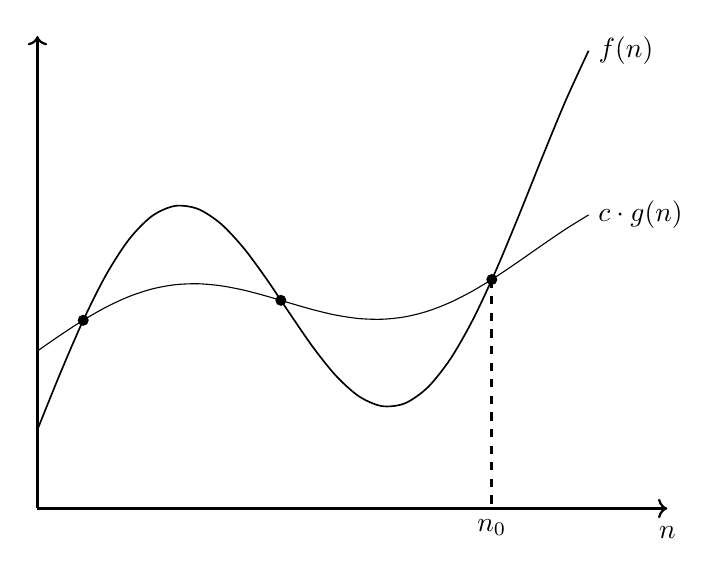
\begin{tikzpicture}
    \draw[->, thick]  (0,0)coordinate(O) -- (8,0) node[anchor=north, yshift=-1mm] {$n$};
    \draw[->, thick]  (0,0) -- (0,6);

\draw[domain=0:7,smooth,variable=\x,semithick,black,name path=c1] plot ({\x},{0.5*\x+2*sin(\x r)+1})node[right, black]{$f(n)$};
\draw[domain=0:7,smooth,variable=\x,black,name path=c2] plot ({\x},{0.2*\x+0.5*sin(\x r)+2})node[right,black]{$c \cdot g(n)$};
\fill[black,name intersections={of=c1 and c2}]
    (intersection-1) circle (2pt)
    (intersection-2) circle (2pt)
        (intersection-3) circle (2pt) ;

\draw[dashed, very thick] (intersection-3) -- (intersection-3|-O) node[below]{$n_0$};
\end{tikzpicture}
\end{center}
\begin{center}
\graytext{$cg$ eventually undetakes $f$}
\end{center}
\end{defboxbot}
\end{frame}


\begin{frame}{Common Complexities}
\vspace{2mm}
Some common complexities include:
\begin{center}

% Row 1
\begin{minipage}{0.23\textwidth}
\centering
\highlight{\textbf{constant}} \\
\graytext{$O(1)$} \\[2mm]
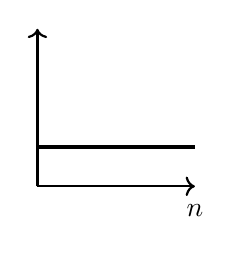
\begin{tikzpicture}[scale=1.0]
\draw[->, thick]  (0,0) -- (2,0) node[anchor=north, yshift=-1mm] {$n$};
\draw[->, thick]  (0,0) -- (0,2);
\clip (0,0) rectangle (2,2);
\draw[domain=0:2,smooth,variable=\x,very thick,black] plot ({\x},{0.5});
\end{tikzpicture}
\end{minipage}%
\hfill
\begin{minipage}{0.23\textwidth}
\centering
\highlight{\textbf{logarithmic}} \\
\graytext{$O(\log n)$} \\[2mm]
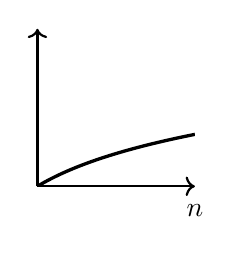
\begin{tikzpicture}[scale=1.0]
\draw[->, thick]  (0,0) -- (2,0) node[anchor=north, yshift=-1mm] {$n$};
\draw[->, thick]  (0,0) -- (0,2);
\clip (0,0) rectangle (2,2);
\draw[domain=0.01:2,smooth,variable=\x,very thick,black] plot ({\x},{0.6*ln(\x+1)});
\end{tikzpicture}
\end{minipage}%
\hfill
\begin{minipage}{0.23\textwidth}
\centering
\highlight{\textbf{linear}} \\
\graytext{$O(n)$} \\[2mm]
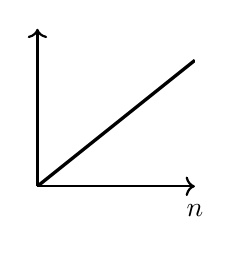
\begin{tikzpicture}[scale=1.0]
\draw[->, thick]  (0,0) -- (2,0) node[anchor=north, yshift=-1mm] {$n$};
\draw[->, thick]  (0,0) -- (0,2);
\clip (0,0) rectangle (2,2);
\draw[domain=0:2,smooth,variable=\x,very thick,black] plot ({\x},{0.8*\x});
\end{tikzpicture}
\end{minipage}%
\hfill
\begin{minipage}{0.23\textwidth}
\centering
\highlight{\textbf{log-linear}} \\
\graytext{$O(n \log n)$} \\[2mm]
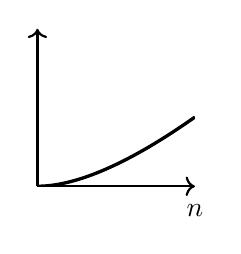
\begin{tikzpicture}[scale=1.0]
\draw[->, thick]  (0,0) -- (2,0) node[anchor=north, yshift=-1mm] {$n$};
\draw[->, thick]  (0,0) -- (0,2);
\clip (0,0) rectangle (2,2);
\draw[domain=0.01:2,smooth,variable=\x,very thick,black] plot ({\x},{0.4*\x*ln(\x+1)});
\end{tikzpicture}
\end{minipage}

\vspace{2mm} % space between rows

% Row 2
\begin{minipage}{0.23\textwidth}
\centering
\highlight{\textbf{quadratic}} \\
\graytext{$O(n^2)$} \\[2mm]
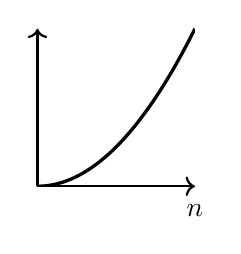
\begin{tikzpicture}[scale=1.0]
\draw[->, thick]  (0,0) -- (2,0) node[anchor=north, yshift=-1mm] {$n$};
\draw[->, thick]  (0,0) -- (0,2);
\clip (0,0) rectangle (2,2);
\draw[domain=0:2,smooth,variable=\x,very thick,black] plot ({\x},{0.5*\x*\x});
\end{tikzpicture}
\end{minipage}%
\hfill
\begin{minipage}{0.23\textwidth}
\centering
\highlight{\textbf{cubic}} \\
\graytext{$O(n^3)$} \\[2mm]
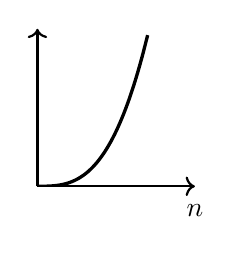
\begin{tikzpicture}[scale=1.0]
\draw[->, thick]  (0,0) -- (2,0) node[anchor=north, yshift=-1mm] {$n$};
\draw[->, thick]  (0,0) -- (0,2);
\clip (0,0) rectangle (2,2);
\draw[domain=0:1.4,smooth,variable=\x,very thick,black] plot ({\x},{0.7*\x*\x*\x});
\end{tikzpicture}
\end{minipage}%
\hfill
\begin{minipage}{0.23\textwidth}
\centering
\highlight{\textbf{exponential}} \\
\graytext{$O(2^n)$} \\[2mm]
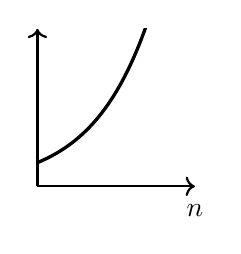
\begin{tikzpicture}[scale=1.0]
\draw[->, thick]  (0,0) -- (2,0) node[anchor=north, yshift=-1mm] {$n$};
\draw[->, thick]  (0,0) -- (0,2);
\clip (0,0) rectangle (2,2);
\draw[domain=0:1.5,smooth,variable=\x,very thick,black] plot ({\x},{0.3*4^\x});
\end{tikzpicture}
\end{minipage}%
\hfill
\begin{minipage}{0.23\textwidth}
\centering
\highlight{\textbf{factorial}} \\
\graytext{$O(n!)$} \\[2mm]
\begin{tikzpicture}[scale=1.0]
\draw[->, thick]  (0,0) -- (2,0) node[anchor=north, yshift=-1mm] {$n$};
\draw[->, thick]  (0,0) -- (0,2);
\clip (0,0) rectangle (2,2);
\draw[domain=0:1.4,smooth,variable=\x,very thick,black] plot ({\x},{0.1*exp(\x*ln(10*\x))}); % approximate factorial growth
\end{tikzpicture}
\end{minipage}

\end{center}
\end{frame}

\begin{frame}[fragile]
\begin{thmboxtop}
\begin{lstlisting}[style=mypython]
class Array:
# attributes
    # the capacity of the array
    capacity: Integer (1)
    # the number of elements currently stored
    size: Integer (0)
    # the array
    array: [None] * self.capacity
\end{lstlisting}
\end{thmboxtop}
\end{frame}

\begin{frame}[fragile]
\begin{thmboxbot}
\begin{lstlisting}[style=mypython, firstnumber=last]
# functions
    # appends an element to the array if there is space;
    # otherwise, doubles the array's capacity before appending
    append(obj: Object) -> Optional[Object]

    def append(self: Array, obj: Object) -> Optional[Object]:
        if self.size is self.capacity:
            self._resize(2 * self.capacity)
        self.array[self.size] = item
        self.size += 1

    def _resize(self: Array, new_capacity: Integer):
        new_array = [None] * new_capacity
        for i in 0, ..., self.size-1:
            new_array[i] = self.array[i]
        self.array = new_array
        self.capacity = new_capacity
\end{lstlisting}
\end{thmboxbot}
\end{frame}

\begin{frame}{Complexity Analysis (Best-Case}
    \begin{center}
        \Large \highlight{\textbf{best-case analysis}} \\[1mm]
        \normalsize\color{gray} (complexity analysis)
    \end{center}
\end{frame}

\begin{frame}{}
\begin{center}
\highlight{\textbf{append}} \\
\graytext{\texttt{Array.append(o3)}}
\end{center}

\begin{figure}
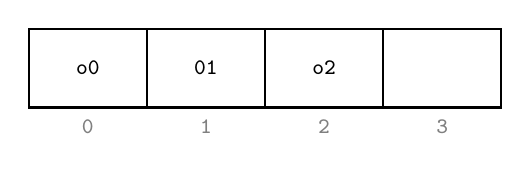
\begin{tikzpicture}

  \node[draw=white, text=black] (l1) at (0,-0.75) {\footnotesize\graytext{\texttt{0}}};
  \node[draw=white, text=black] (l2) at (1.5, -0.75) {\footnotesize\graytext{\texttt{1}}};
  \node[draw=white, text=black] (l3) at (3,-0.75) {\footnotesize\graytext{\texttt{2}}};
  \node[draw=white, text=black] (l4) at (4.5,-0.75) {\footnotesize\graytext{\texttt{3}}};

  \node[defaultnode, arraynode] (m1) at (0,0) {};
  \node[defaultnode, arraynode] (m2) at (1.5,0) {};
  \node[defaultnode, arraynode] (m3) at (3,0) {};
  \node[defaultnode, arraynode] (m4) at (4.5,0) {};

  \node at (m1) {\footnotesize\texttt{o0}};
  \node at (m2) {\footnotesize\texttt{01}};
  \node at (m3) {\footnotesize\texttt{o2}};

\end{tikzpicture}
\end{figure}

\begin{center}
\graytext{an array before \texttt{Array.append(o3)} is called}
\end{center}
\end{frame}

\begin{frame}{}
\begin{center}
\highlight{\textbf{append}} \\
\graytext{\texttt{Array.append(o3)}}
\end{center}

\begin{figure}
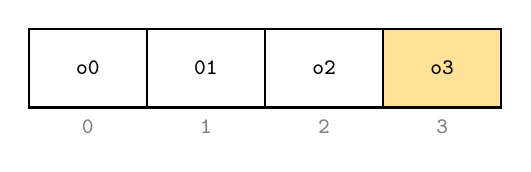
\begin{tikzpicture}

  \node[draw=white, text=black] (l1) at (0,-0.75) {\footnotesize\graytext{\texttt{0}}};
  \node[draw=white, text=black] (l2) at (1.5, -0.75) {\footnotesize\graytext{\texttt{1}}};
  \node[draw=white, text=black] (l3) at (3,-0.75) {\footnotesize\graytext{\texttt{2}}};
  \node[draw=white, text=black] (l4) at (4.5,-0.75) {\footnotesize\graytext{\texttt{3}}};

  \node[defaultnode, arraynode] (m1) at (0,0) {};
  \node[defaultnode, arraynode] (m2) at (1.5,0) {};
  \node[defaultnode, arraynode] (m3) at (3,0) {};
  \node[newnode, draw=black, arraynode] (m4) at (4.5,0) {};

  \node at (m1) {\footnotesize\texttt{o0}};
  \node at (m2) {\footnotesize\texttt{01}};
  \node at (m3) {\footnotesize\texttt{o2}};
  \node at (m4) {\footnotesize\texttt{o3}};

\end{tikzpicture}
\end{figure}

\begin{center}
\graytext{the array after \texttt{Array.append(o3)} is called}
\end{center}
\end{frame}

\begin{frame}{Complexity Analysis (Worst-Case}
    \begin{center}
        \Large \highlight{\textbf{worst-case analysis}} \\[1mm]
        \normalsize\color{gray} (complexity analysis)
    \end{center}
\end{frame}

\begin{frame}{}
\begin{center}
\highlight{\textbf{append}} \\
\graytext{\texttt{Array.append(o4)}}
\end{center}

\begin{figure}
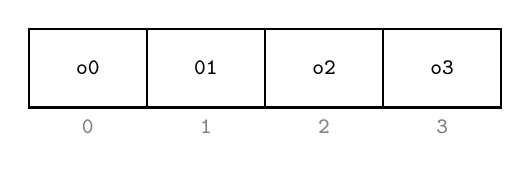
\begin{tikzpicture}

  \node[draw=white, text=black] (l1) at (0,-0.75) {\footnotesize\graytext{\texttt{0}}};
  \node[draw=white, text=black] (l2) at (1.5, -0.75) {\footnotesize\graytext{\texttt{1}}};
  \node[draw=white, text=black] (l3) at (3,-0.75) {\footnotesize\graytext{\texttt{2}}};
  \node[draw=white, text=black] (l4) at (4.5,-0.75) {\footnotesize\graytext{\texttt{3}}};

  \node[defaultnode, arraynode] (m1) at (0,0) {};
  \node[defaultnode, arraynode] (m2) at (1.5,0) {};
  \node[defaultnode, arraynode] (m3) at (3,0) {};
  \node[defaultnode, arraynode] (m4) at (4.5,0) {};

  \node at (m1) {\footnotesize\texttt{o0}};
  \node at (m2) {\footnotesize\texttt{01}};
  \node at (m3) {\footnotesize\texttt{o2}};
  \node at (m4) {\footnotesize\texttt{o3}};

\end{tikzpicture}
\end{figure}

\begin{center}
\graytext{an array before \texttt{Array.append(o4)} is called}
\end{center}
\end{frame}

\begin{frame}{}
\begin{center}
\highlight{\textbf{append}} \\
\graytext{\texttt{Array.append(o4)}}
\end{center}

\begin{figure}
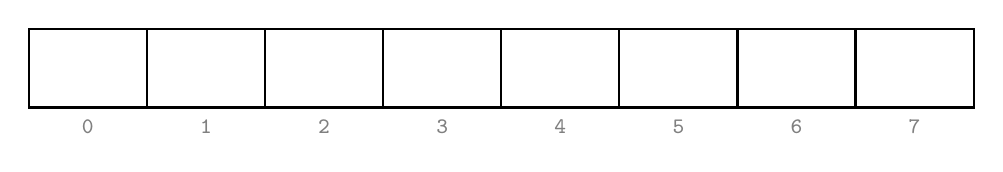
\begin{tikzpicture}

  \node[draw=white, text=black] (l1) at (0,-0.75) {\footnotesize\graytext{\texttt{0}}};
  \node[draw=white, text=black] (l2) at (1.5, -0.75) {\footnotesize\graytext{\texttt{1}}};
  \node[draw=white, text=black] (l3) at (3,-0.75) {\footnotesize\graytext{\texttt{2}}};
  \node[draw=white, text=black] (l4) at (4.5,-0.75) {\footnotesize\graytext{\texttt{3}}};
    \node[draw=white, text=black] (l1) at (6,-0.75) {\footnotesize\graytext{\texttt{4}}};
  \node[draw=white, text=black] (l2) at (7.5, -0.75) {\footnotesize\graytext{\texttt{5}}};
  \node[draw=white, text=black] (l3) at (9,-0.75) {\footnotesize\graytext{\texttt{6}}};
  \node[draw=white, text=black] (l4) at (10.5,-0.75) {\footnotesize\graytext{\texttt{7}}};

  \node[defaultnode, arraynode] (m1) at (0,0) {};
  \node[defaultnode, arraynode] (m2) at (1.5,0) {};
  \node[defaultnode, arraynode] (m3) at (3,0) {};
  \node[defaultnode, arraynode] (m4) at (4.5,0) {};
  \node[defaultnode, arraynode] (m5) at (6,0) {};
  \node[defaultnode, arraynode] (m6) at (7.5,0) {};
  \node[defaultnode, arraynode] (m7) at (9,0) {};
  \node[defaultnode, arraynode] (m8) at (10.5,0) {};

\end{tikzpicture}
\end{figure}

\begin{center}
\graytext{the array during \texttt{Array.append(o4)} (resized)}
\end{center}
\end{frame}

\begin{frame}{}
\begin{center}
\highlight{\textbf{append}} \\
\graytext{\texttt{Array.append(o4)}}
\end{center}

\begin{figure}
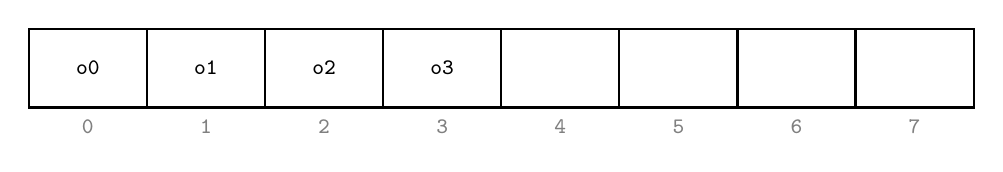
\begin{tikzpicture}

  \node[draw=white, text=black] (l1) at (0,-0.75) {\footnotesize\graytext{\texttt{0}}};
  \node[draw=white, text=black] (l2) at (1.5, -0.75) {\footnotesize\graytext{\texttt{1}}};
  \node[draw=white, text=black] (l3) at (3,-0.75) {\footnotesize\graytext{\texttt{2}}};
  \node[draw=white, text=black] (l4) at (4.5,-0.75) {\footnotesize\graytext{\texttt{3}}};
    \node[draw=white, text=black] (l1) at (6,-0.75) {\footnotesize\graytext{\texttt{4}}};
  \node[draw=white, text=black] (l2) at (7.5, -0.75) {\footnotesize\graytext{\texttt{5}}};
  \node[draw=white, text=black] (l3) at (9,-0.75) {\footnotesize\graytext{\texttt{6}}};
  \node[draw=white, text=black] (l4) at (10.5,-0.75) {\footnotesize\graytext{\texttt{7}}};

  \node[defaultnode, arraynode] (m1) at (0,0) {};
  \node[defaultnode, arraynode] (m2) at (1.5,0) {};
  \node[defaultnode, arraynode] (m3) at (3,0) {};
  \node[defaultnode, arraynode] (m4) at (4.5,0) {};
  \node[defaultnode, arraynode] (m5) at (6,0) {};
  \node[defaultnode, arraynode] (m6) at (7.5,0) {};
  \node[defaultnode, arraynode] (m7) at (9,0) {};
  \node[defaultnode, arraynode] (m8) at (10.5,0) {};

  \node at (m1) {\footnotesize\texttt{o0}};
  \node at (m2) {\footnotesize\texttt{o1}};
  \node at (m3) {\footnotesize\texttt{o2}};
  \node at (m4) {\footnotesize\texttt{o3}};

\end{tikzpicture}
\end{figure}

\begin{center}
\graytext{the array during \texttt{Array.append(o4)} (old elements copied)}
\end{center}
\end{frame}

\begin{frame}{}
\begin{center}
\highlight{\textbf{append}} \\
\graytext{\texttt{Array.append(o4)}}
\end{center}

\begin{figure}
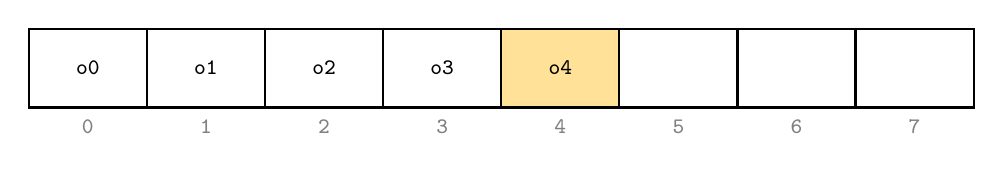
\begin{tikzpicture}

  \node[draw=white, text=black] (l1) at (0,-0.75) {\footnotesize\graytext{\texttt{0}}};
  \node[draw=white, text=black] (l2) at (1.5, -0.75) {\footnotesize\graytext{\texttt{1}}};
  \node[draw=white, text=black] (l3) at (3,-0.75) {\footnotesize\graytext{\texttt{2}}};
  \node[draw=white, text=black] (l4) at (4.5,-0.75) {\footnotesize\graytext{\texttt{3}}};
    \node[draw=white, text=black] (l1) at (6,-0.75) {\footnotesize\graytext{\texttt{4}}};
  \node[draw=white, text=black] (l2) at (7.5, -0.75) {\footnotesize\graytext{\texttt{5}}};
  \node[draw=white, text=black] (l3) at (9,-0.75) {\footnotesize\graytext{\texttt{6}}};
  \node[draw=white, text=black] (l4) at (10.5,-0.75) {\footnotesize\graytext{\texttt{7}}};

  \node[defaultnode, arraynode] (m1) at (0,0) {};
  \node[defaultnode, arraynode] (m2) at (1.5,0) {};
  \node[defaultnode, arraynode] (m3) at (3,0) {};
  \node[defaultnode, arraynode] (m4) at (4.5,0) {};
  \node[newnode, arraynode, draw=black] (m5) at (6,0) {};
  \node[defaultnode, arraynode] (m6) at (7.5,0) {};
  \node[defaultnode, arraynode] (m7) at (9,0) {};
  \node[defaultnode, arraynode] (m8) at (10.5,0) {};

  \node at (m1) {\footnotesize\texttt{o0}};
  \node at (m2) {\footnotesize\texttt{o1}};
  \node at (m3) {\footnotesize\texttt{o2}};
  \node at (m4) {\footnotesize\texttt{o3}};
  \node at (m5) {\footnotesize\texttt{o4}};

\end{tikzpicture}
\end{figure}

\begin{center}
\graytext{the array after \texttt{Array.append(o4)}}
\end{center}
\end{frame}


\begin{frame}{Complexity Analysis (Average-Case}
    \begin{center}
        \Large \highlight{\textbf{average-case analysis}} \\[1mm]
        \normalsize\color{gray} (complexity analysis)
    \end{center}
\end{frame}


\begin{frame}{Amortized Complexity}
\begin{center}
\Large \highlight{\textbf{amortized case}} \\[1mm]
\normalsize\color{gray} (complexity analysis)
\end{center}
\end{frame}

\begin{frame}
Many algorithms are often cheap but occasionally expensive.
\\[8mm]
\begin{minipage}{0.33\textwidth}
\centering
\highlight{\textbf{worst-case}} \\[2mm]
\footnotesize\textcolor{gray}{can be too pessimistic}
\end{minipage}%
\begin{minipage}{0.33\textwidth}
\centering
\highlight{\textbf{best-case}} \\[2mm]
\footnotesize\textcolor{gray}{can be too optimistic}
\end{minipage}%
\begin{minipage}{0.33\textwidth}
\centering
\highlight{\textbf{average-case}} \\[2mm]
\footnotesize\textcolor{gray}{often hard to compute}
\end{minipage}
\\[8mm]
We need a way to measure the long-term cost per call of the algorithm.
\end{frame}

\begin{frame}{}
\begin{center}
\highlight{\textbf{append}} \\
\graytext{\texttt{Array.append(o1)}, $\dots$, \texttt{Array.append(o8)}}
\end{center}

\begin{figure}
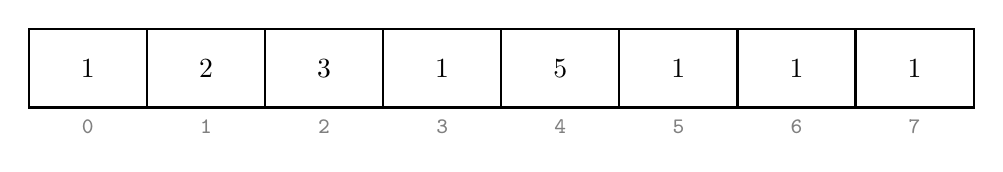
\begin{tikzpicture}

  \node[draw=white, text=black] (l1) at (0,-0.75) {\footnotesize\graytext{\texttt{0}}};
  \node[draw=white, text=black] (l2) at (1.5, -0.75) {\footnotesize\graytext{\texttt{1}}};
  \node[draw=white, text=black] (l3) at (3,-0.75) {\footnotesize\graytext{\texttt{2}}};
  \node[draw=white, text=black] (l4) at (4.5,-0.75) {\footnotesize\graytext{\texttt{3}}};
    \node[draw=white, text=black] (l1) at (6,-0.75) {\footnotesize\graytext{\texttt{4}}};
  \node[draw=white, text=black] (l2) at (7.5, -0.75) {\footnotesize\graytext{\texttt{5}}};
  \node[draw=white, text=black] (l3) at (9,-0.75) {\footnotesize\graytext{\texttt{6}}};
  \node[draw=white, text=black] (l4) at (10.5,-0.75) {\footnotesize\graytext{\texttt{7}}};

  \node[defaultnode, arraynode] (m1) at (0,0) {1};
  \node[defaultnode, arraynode] (m2) at (1.5,0) {2};
  \node[defaultnode, arraynode] (m3) at (3,0) {3};
  \node[defaultnode, arraynode] (m4) at (4.5,0) {1};
  \node[defaultnode, arraynode] (m5) at (6,0) {5};
  \node[defaultnode, arraynode] (m6) at (7.5,0) {1};
  \node[defaultnode, arraynode] (m7) at (9,0) {1};
  \node[defaultnode, arraynode] (m8) at (10.5,0) {1};

\end{tikzpicture}
\end{figure}

\begin{center}
\graytext{the complexity of \texttt{Array.append($\cdot$)} for the $m$\textsuperscript{th} call}
\end{center}
\end{frame}



\begin{frame}
\vspace{-2mm}
\begin{proofbox}
\highlight{\textbf{aggregate method}}: \\
\graytext{(amortized complexity analysis)} \\[-2mm]
\begin{enumerate}
\item \highlight{\textbf{define complexity function}} \\
\graytext{define $T(m)$ as the complexity of the $m$\textsuperscript{th} successive call of the algorithm}
\item \highlight{\textbf{compute amortized complexity}} \\
\graytext{average $T(m)$ from $m = 1$ to $M$}
\[\hat{T}(M) = \frac{1}{M}\sum_{n=1}^{M}T(m)\]
\end{enumerate}
\end{proofbox}
\end{frame}

\begin{frame}
    \begin{thmbox}
    Suppose \texttt{append} is called $M$ times. Let $T(m)$ denote the complexity of the $m$\textsuperscript{th} \texttt{append} call:
        \[T(m) = \begin{cases} m & \log_2(m) \in \mathbb{N} \\ 1 & \text{otherwise}\end{cases}\]
            This is because the array must be resized on calls  $1, 2, 4, \dots 2^{\floor{\log_2(M)}}$, or equivalently whenever $\log_2(m) \in \mathbb{N}$. Therefore,
            \begin{align*}
            \bar{T}(M) &= \sum_{\substack{m = 1 \\ \log_2(m) \in \mathbb{N}}}^{M}m + \sum_{\substack{m=1 \\ \log_2(m) \not\in \mathbb{N}}}^{M} 1\\
            &\leq M+\left(1+2+4+\dots+2^{{\log_2(M)}}\right) \\
            &= M+2M-1
            \end{align*}
    \end{thmbox}
\end{frame}

\begin{frame}
\vspace{-2mm}
\begin{proofbox}
\highlight{\textbf{accounting method}}: \\
\graytext{(amortized complexity analysis)} \\[-6mm]
\begin{minipage}{0.32\textwidth}
\centering
\begin{tikzpicture}
\node at (0,0) {
\includegraphics[scale=0.1]{images/price_tag.png}};
\node at (0,0) {$1^{00}$};
\draw[opacity=0] (-2,-0.75) rectangle (2,2);
\end{tikzpicture}
\color{gray}(1) \color{black} \highlight{\textbf{set prices}} \\[1mm]
\footnotesize\color{gray} 
charge each call a cost based on its complexity

\end{minipage}
\hfill
\begin{minipage}{0.32\textwidth}
\centering
\begin{tikzpicture}
\node at (-0.3,-0.3) {
\includegraphics[scale=0.04]{images/stone_coin.png}};
\node at (0.3,0.3) {
\includegraphics[scale=0.04]{images/stone_coin.png}};
\draw[opacity=0] (-2,-0.75) rectangle (2,2);
\end{tikzpicture}
\color{gray}(2) \color{black} \highlight{\textbf{make payments}} \\[1mm]
\footnotesize\color{gray} 
store extra payments \\ as credits
\end{minipage}
\hfill
\begin{minipage}{0.32\textwidth}
\centering
\begin{tikzpicture}
\node at (0,0) {
\includegraphics[scale=0.04]{images/stone_coin.png}};
\draw[opacity=0] (-2,-1.1) rectangle (2,2);
\end{tikzpicture}
\color{gray}(3) \color{black} \highlight{\textbf{use credits}} \\[1mm]
\footnotesize\color{gray} 
use credits to \\ cover calls
\end{minipage}
\\[5mm]
\color{gray}(4) \color{black} \highlight{\textbf{show balance}} \\
\graytext{show that payments are sufficient to ensure balance is never negative}
\end{proofbox}
\end{frame}


\begin{frame}
\highlight{\textbf{set prices}} \\[1mm]
\footnotesize\color{gray} 
charge each call based on the number of array accesses required
\begin{figure}
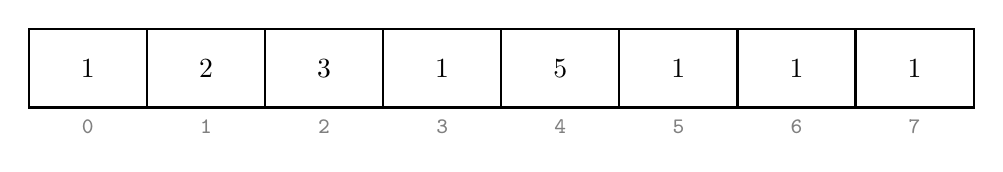
\begin{tikzpicture}

    \node[draw=white, text=black] (l1) at (0,-0.75) {\footnotesize\graytext{\texttt{0}}};
    \node[draw=white, text=black] (l2) at (1.5, -0.75) {\footnotesize\graytext{\texttt{1}}};
    \node[draw=white, text=black] (l3) at (3,-0.75) {\footnotesize\graytext{\texttt{2}}};
    \node[draw=white, text=black] (l4) at (4.5,-0.75) {\footnotesize\graytext{\texttt{3}}};
    \node[draw=white, text=black] (l1) at (6,-0.75) {\footnotesize\graytext{\texttt{4}}};
    \node[draw=white, text=black] (l2) at (7.5, -0.75) {\footnotesize\graytext{\texttt{5}}};
    \node[draw=white, text=black] (l3) at (9,-0.75) {\footnotesize\graytext{\texttt{6}}};
    \node[draw=white, text=black] (l4) at (10.5,-0.75) {\footnotesize\graytext{\texttt{7}}};
    
  \node[defaultnode, arraynode] (m1) at (0,0) {1};
  \node[defaultnode, arraynode] (m2) at (1.5,0) {2};
  \node[defaultnode, arraynode] (m3) at (3,0) {3};
  \node[defaultnode, arraynode] (m4) at (4.5,0) {1};
  \node[defaultnode, arraynode] (m5) at (6,0) {5};
  \node[defaultnode, arraynode] (m6) at (7.5,0) {1};
  \node[defaultnode, arraynode] (m7) at (9,0) {1};
  \node[defaultnode, arraynode] (m8) at (10.5,0) {1};

\end{tikzpicture}
\end{figure}
\normalsize\color{black}
    \highlight{\textbf{make payments}} / \highlight{\textbf{use credits}} \\[1mm]
    \footnotesize\color{gray} 
    pay 3 \scalebox{0.85}{\raisebox{-0.3\height}{
\includegraphics[scale=0.02]{images/stone_coin.png}}} for each call and store extra payments credits
\normalsize
\begin{figure}
    \centering
    \begin{tikzpicture}[every node/.style={shape=rectangle,
draw=black,
thick,
minimum size=10mm,
inner sep=0pt}]

\node[draw=white, text=black] (l1) at (0,0.5) {\footnotesize\graytext{\texttt{0}}};
    \node[draw=white, text=black] (l2) at (1.5, 0.5) {\footnotesize\graytext{\texttt{1}}};
    \node[draw=white, text=black] (l3) at (3,0.5) {\footnotesize\graytext{\texttt{2}}};
    \node[draw=white, text=black] (l4) at (4.5,0.5) {\footnotesize\graytext{\texttt{3}}};
    \node[draw=white, text=black] (l1) at (6,0.5) {\footnotesize\graytext{\texttt{4}}};
    \node[draw=white, text=black] (l2) at (7.5, 0.5) {\footnotesize\graytext{\texttt{5}}};
    \node[draw=white, text=black] (l3) at (9,0.5) {\footnotesize\graytext{\texttt{6}}};
    \node[draw=white, text=black] (l4) at (10.5,0.5) {\footnotesize\graytext{\texttt{7}}};
    

\node[draw opacity=0] (c) at (0,1) {
\includegraphics[scale=0.04]{images/coin_side.png}};
\node[draw opacity=0] (c) at (0,1.1) {
\includegraphics[scale=0.04]{images/coin_side.png}};

\node[draw opacity=0] (c) at (1.5,1) {
\includegraphics[scale=0.04]{images/coin_side.png}};
\node[draw opacity=0] (c) at (1.5,1.1) {
\includegraphics[scale=0.04]{images/coin_side.png}};
\node[draw opacity=0] (c) at (1.5,1.2) {
\includegraphics[scale=0.04]{images/coin_side.png}};

\node[draw opacity=0] (c) at (3,1) {
\includegraphics[scale=0.04]{images/coin_side.png}};
\node[draw opacity=0] (c) at (3,1.1) {
\includegraphics[scale=0.04]{images/coin_side.png}};
\node[draw opacity=0] (c) at (3,1.2) {
\includegraphics[scale=0.04]{images/coin_side.png}};

\node[draw opacity=0] (c) at (4.5,1) {
\includegraphics[scale=0.04]{images/coin_side.png}};
\node[draw opacity=0] (c) at (4.5,1.1) {
\includegraphics[scale=0.04]{images/coin_side.png}};
\node[draw opacity=0] (c) at (4.5,1.2) {
\includegraphics[scale=0.04]{images/coin_side.png}};
\node[draw opacity=0] (c) at (4.5,1.3) {
\includegraphics[scale=0.04]{images/coin_side.png}};
\node[draw opacity=0] (c) at (4.5,1.4) {
\includegraphics[scale=0.04]{images/coin_side.png}};

\node[draw opacity=0] (c) at (6,1) {
\includegraphics[scale=0.04]{images/coin_used.png}};
\node[draw opacity=0] (c) at (6,1.1) {
\includegraphics[scale=0.04]{images/coin_used.png}};
\node[draw opacity=0] (c) at (6,1.2) {
\includegraphics[scale=0.04]{images/coin_used.png}};
\node[draw opacity=0] (c) at (6,1.3) {
\includegraphics[scale=0.04]{images/coin_used.png}};
\node[draw opacity=0] (c) at (6,1.4) {
\includegraphics[scale=0.04]{images/coin_used.png}};
\node[draw opacity=0] (c) at (6,1.5) {
\includegraphics[scale=0.04]{images/coin_side.png}};
\node[draw opacity=0] (c) at (6,1.6) {
\includegraphics[scale=0.04]{images/coin_side.png}};
\node[draw opacity=0] (c) at (6,1.7) {
\includegraphics[scale=0.04]{images/coin_side.png}};

\node[draw opacity=0] (c) at (7.5,1) {
\includegraphics[scale=0.04]{images/coin_side.png}};
\node[draw opacity=0] (c) at (7.5,1.1) {
\includegraphics[scale=0.04]{images/coin_side.png}};
\node[draw opacity=0] (c) at (7.5,1.2) {
\includegraphics[scale=0.04]{images/coin_side.png}};
\node[draw opacity=0] (c) at (7.5,1.3) {
\includegraphics[scale=0.04]{images/coin_side.png}};
\node[draw opacity=0] (c) at (7.5,1.4) {
\includegraphics[scale=0.04]{images/coin_side.png}};

\node[draw opacity=0] (c) at (9,1) {
\includegraphics[scale=0.04]{images/coin_side.png}};
\node[draw opacity=0] (c) at (9,1.1) {
\includegraphics[scale=0.04]{images/coin_side.png}};
\node[draw opacity=0] (c) at (9,1.2) {
\includegraphics[scale=0.04]{images/coin_side.png}};
\node[draw opacity=0] (c) at (9,1.3) {
\includegraphics[scale=0.04]{images/coin_side.png}};
\node[draw opacity=0] (c) at (9,1.4) {
\includegraphics[scale=0.04]{images/coin_side.png}};
\node[draw opacity=0] (c) at (9,1.5) {
\includegraphics[scale=0.04]{images/coin_side.png}};
\node[draw opacity=0] (c) at (9,1.6) {
\includegraphics[scale=0.04]{images/coin_side.png}};

\node[draw opacity=0] (c) at (10.5,1) {
\includegraphics[scale=0.04]{images/coin_side.png}};
\node[draw opacity=0] (c) at (10.5,1.1) {
\includegraphics[scale=0.04]{images/coin_side.png}};
\node[draw opacity=0] (c) at (10.5,1.2) {
\includegraphics[scale=0.04]{images/coin_side.png}};
\node[draw opacity=0] (c) at (10.5,1.3) {
\includegraphics[scale=0.04]{images/coin_side.png}};
\node[draw opacity=0] (c) at (10.5,1.4) {
\includegraphics[scale=0.04]{images/coin_side.png}};
\node[draw opacity=0] (c) at (10.5,1.5) {
\includegraphics[scale=0.04]{images/coin_side.png}};
\node[draw opacity=0] (c) at (10.5,1.6) {
\includegraphics[scale=0.04]{images/coin_side.png}};
\node[draw opacity=0] (c) at (10.5,1.7) {
\includegraphics[scale=0.04]{images/coin_side.png}};
\node[draw opacity =0] (c) at (10.5,1.8) {
\includegraphics[scale=0.04]{images/coin_side.png}};

\end{tikzpicture}
\end{figure}
\vspace{-2mm}
\color{black}
\highlight{\textbf{show balance}}\\
\graytext{the balance will never be negative}

\end{frame}

\end{document}